\begin{paracol}{2}
\begin{leftcolumn}
%\fcolorbox{white}{white}{
%\begin{minipage}[c][0.95\textheight][t]{\linewidth}


%---------------------------------------------------------------------------------------
%	TITLE HEADLINE
%----------------------------------------------------------------------------------------
\vspace{-3pt}
% use this for multiple words like working titles etc.
%\hspace{-0.25\linewidth}\colorbox{bgcol}{\makebox[1.5\linewidth][c]{\hspace{46pt}\HUGE{\textcolor{white}{\uppercase{M.Sc. Jan Küster}} } \textcolor{sectcol}{\rule[-1mm]{1mm}{0.9cm}} \parbox[b]{5cm}{   \large{ \textcolor{white}{{IT Consultant}}}\\
% \large{ \textcolor{white}{{JS Fullstack Engineer}}}}
%}}

% use this for single words, e.g. CV or RESUME etc.
\colorbox{bgcol}{\makebox[\linewidth][c]{\HUGE{\textcolor{white}{\uppercase{Jérémie Libeau}} } \textcolor{sectcol}{\rule[-1mm]{1mm}{0.9cm}} \HUGE{\textcolor{white}{\uppercase{CV}} } }}

%----------------------------------------------------------------------------------------
%	HEADER IMAGE
%----------------------------------------------------------------------------------------


%\hspace{-1.6cm}
%\includegraphics[trim= 0 250 0 270,clip,width=1\linewidth+3.1cm]{myfoto.jpg}	%trimming relative to image size!
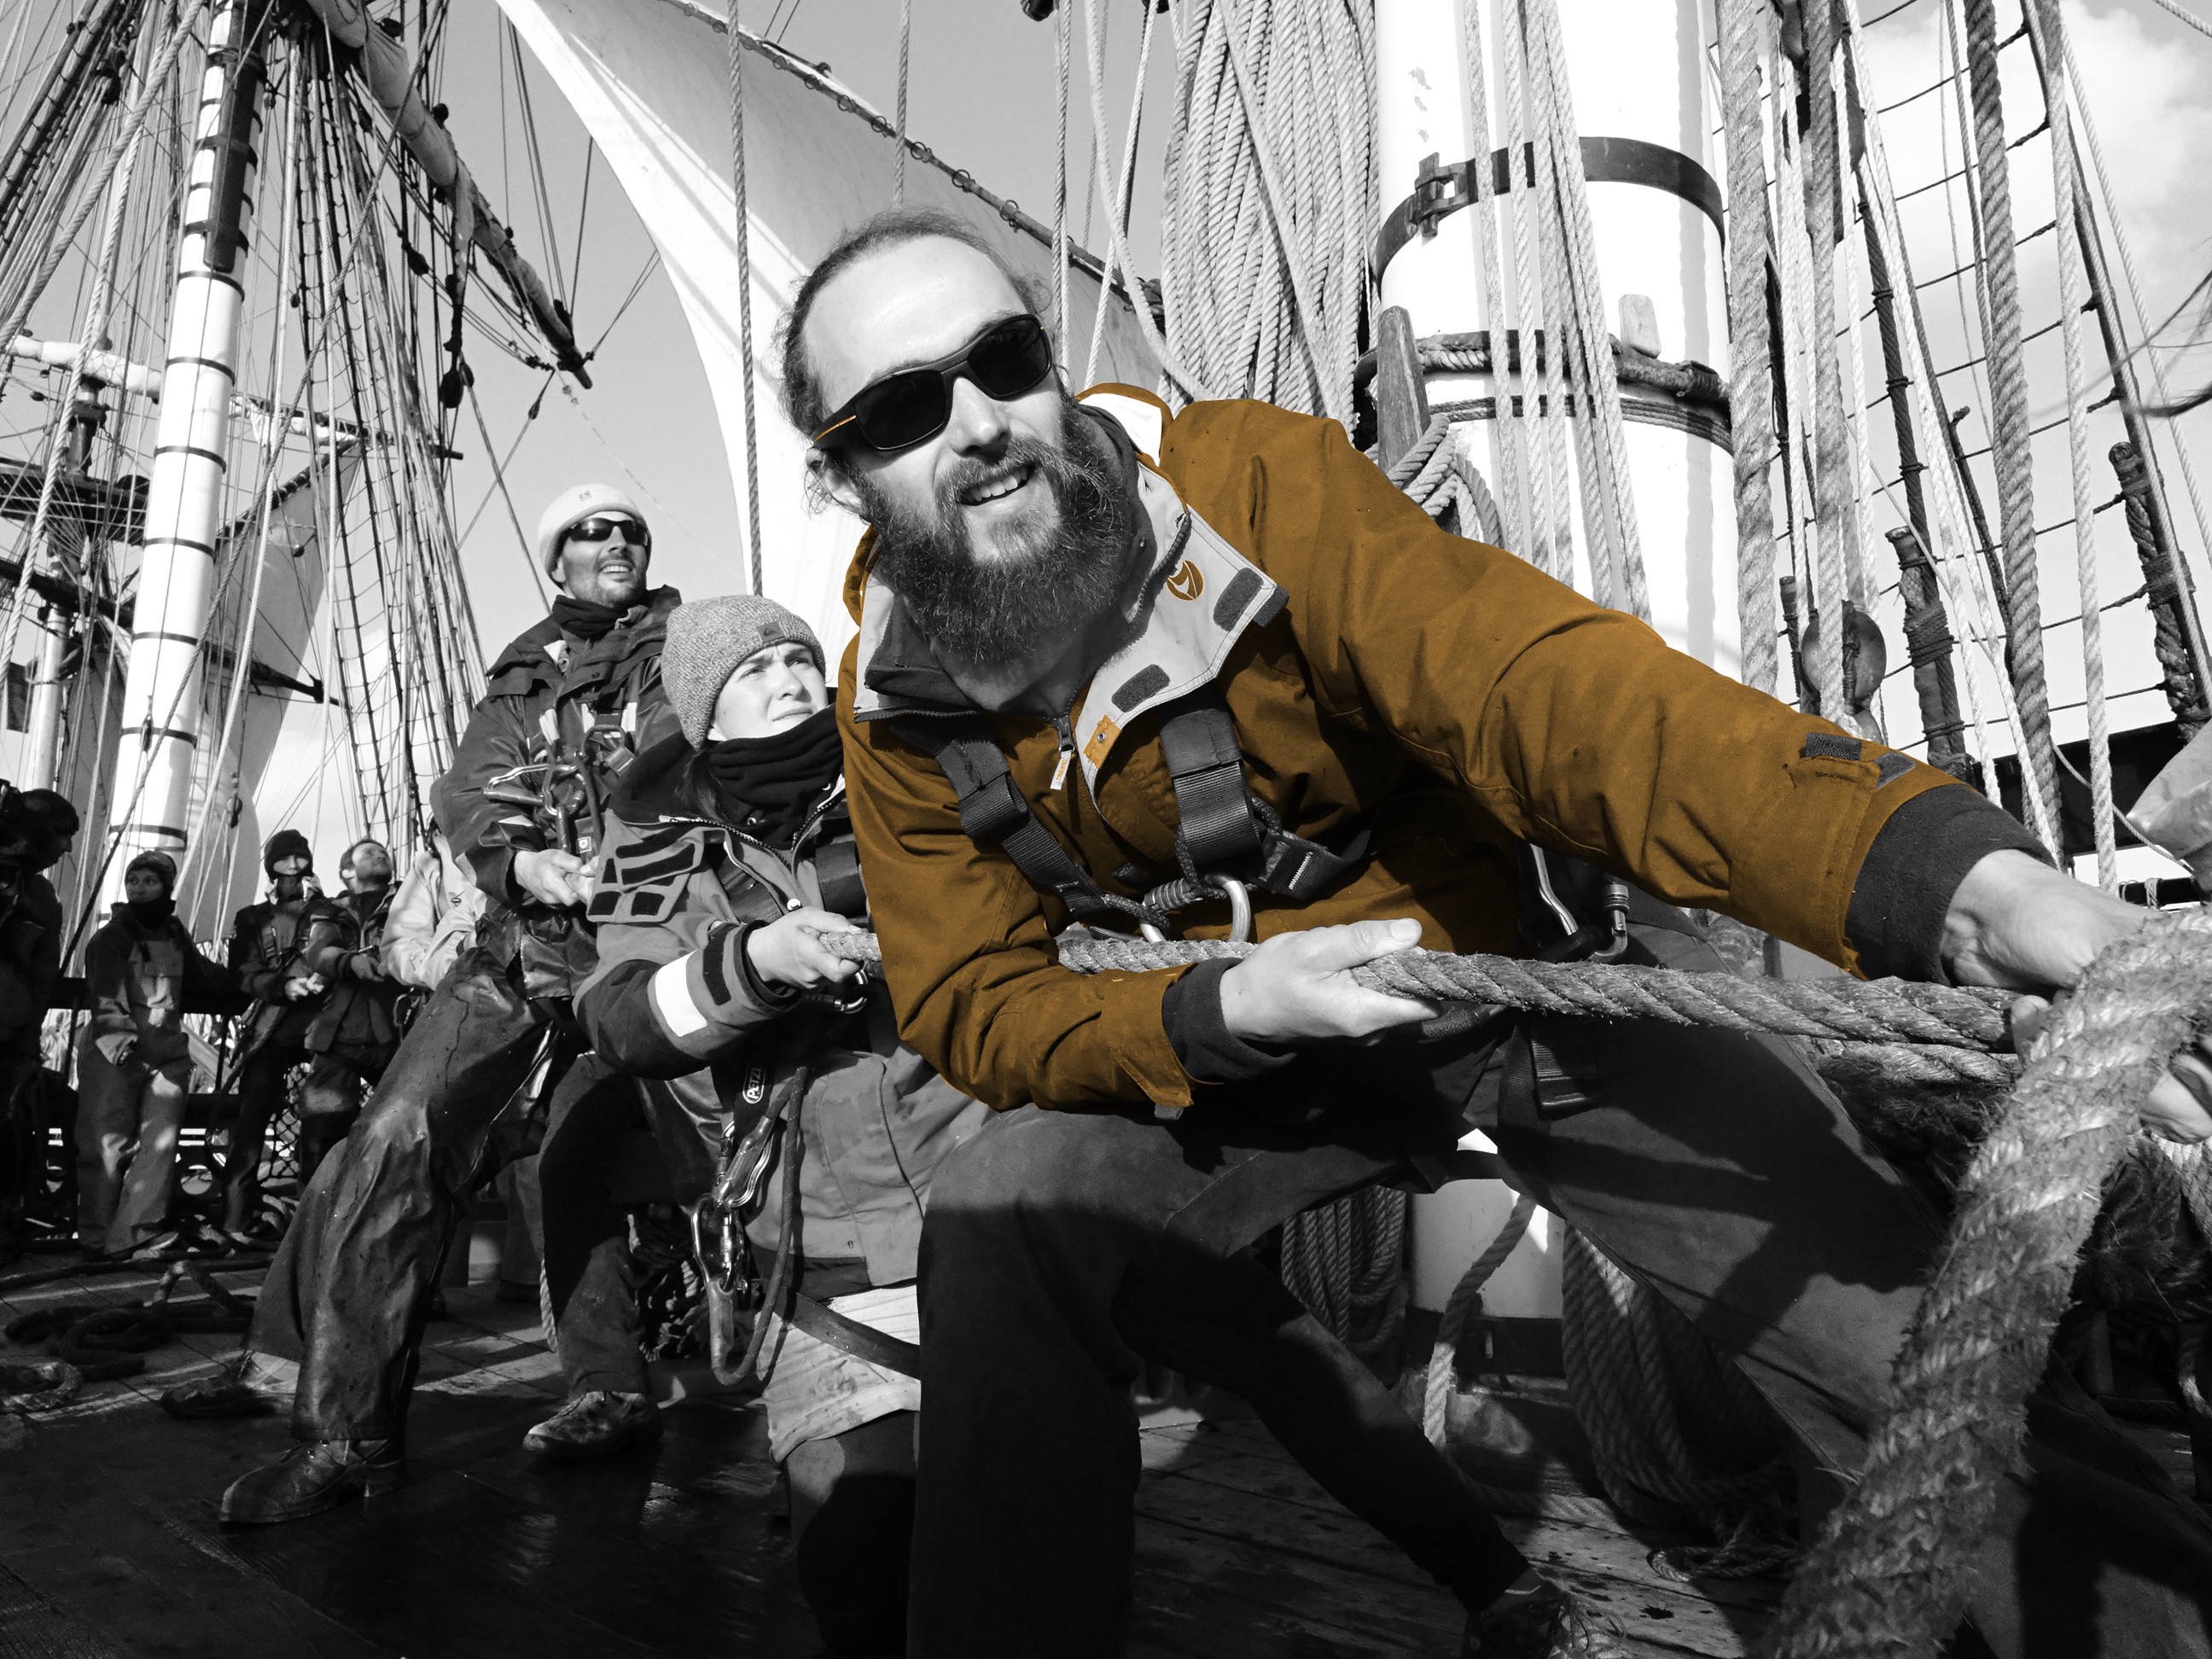
\includegraphics[trim= 100 150 0 40, clip ,width=\linewidth+5px]{images/photo.jpg}	%trimming relative to image size

%---------------------------------------------------------------------------------------
%	SUMMARY
%----------------------------------------------------------------------------------------
\transparent{0.85}%
\vspace{-180pt}
\hspace{0.59\linewidth}
\colorbox{bgcol}{
	\parbox{0.35\linewidth}{
		\transparent{1}%
		\begin{center}
		\tzlbrace{sectcol}\textcolor{white}{Talk | Think | Create}\tzrbrace{sectcol}
		\end{center}
	}
}
\vspace{145pt}

%============================================================================%
%
%	CV SECTIONS AND EVENTS (MAIN CONTENT)
%
%============================================================================%

%---------------------------------------------------------------------------------------
%	STATUS
%----------------------------------------------------------------------------------------
\cvsection{Status}

Fullstack Developer | Tech Lead

\vspace{12pt}

%---------------------------------------------------------------------------------------
%	EDUCATION SECTION
%--------------------------------------------------------------------------------------
\cvsection{Education}

\cvevent{2010}{Diplôme d'expert en ingénierie informatique --- Master's level}{Epita}{Kremlin-Bicêtre}{
	Computer Engineering Expert Degree,
	Apprenticeship at Siemens Mobility in Châtillon}

\cvevent{2007}{DUT Informatique}{IUT de Vannes}{}{
	Associate Degree in Computer Science,
	Software Engineering option}

\cvevent{2005}{Baccalauréat Scientifique --- mention Assez Bien}{Lycée Chevrollier}{Angers}{
	Scientific Baccalaureate --- with honors,
	Engineering Sciences specialization}

\vspace{12pt}

%---------------------------------------------------------------------------------------
%	EXPERIENCE
%----------------------------------------------------------------------------------------
\cvsection{Experience}

\cvevent{2026/03}{Fullstack Developer --- freelance}{Astrolabe}{Rennes \emph{remote}}{
	Fullstack development in \emph{PHP} and \emph{React}
}

\cvevent{2023/03 - 2025/12}{Tech lead}{EGERIE}{Toulon \emph{remote}}{
    Backend development in \emph{PHP}{,} \emph{Silex} and \emph{Symfony} frameworks,
	\emph{React} development,
    Backend chapter coordination,
    Setup and follow-up of code quality best practices: \emph{clean code}{,} \emph{SOLID},
    Design of a \emph{Hexagonal} architecture with \emph{API Platform},
    Writing \emph{ADRs} discussed in \emph{guild},
    Technical mentoring of developers,
    Unit and functional testing with \emph{PHPUnit}
}

\cvevent{2018/01 - 2023/03}{Fullstack Developer / DevOps}{Symetri}{Rennes}{
	Backend in \emph{PHP}{,} \emph{Symfony} and \emph{Zend} frameworks{,} \emph{MSSql} database,
	Web frontend in \emph{JS} with \emph{Angular} framework,
	Administration of the OBS cloud production platform,
	Unit and functional testing with \emph{PHPUnit},
	Setup of a CI/CD platform with \emph{Jenkins} then \emph{Gitlab},
	Dockerization of applications and setup of a \emph{Kubernetes} infrastructure,
	Participation in \emph{SCRUM} project coordination}

\cvevent{2014/05 - 2017/12}{Fullstack Developer}{Avenue du Web}{Rennes}{
	Backend in \emph{PHP} with \emph{Symfony 2} framework{,} \emph{MySQL} database,
	Development of a live web comment system{,} based on websockets,
	JS frontend,
	Administration of development tools,
	Unit and functional testing with \emph{PHPUnit},
	Setup of an automated testing platform with \emph{Jenkins},
	Participation in \emph{SCRUM} project coordination}

\cvevent{2013/06 - 2014/03}{Fullstack Developer}{Outscale}{Saint-Cloud}{
	Development with \emph{PHP} \emph{Silex} and \emph{RubyOnRails},
	Development and integration of reporting and billing software,
	Technical documentation,
	Participation in \emph{SCRUM} project coordination}

\cvevent{2011/08 - 2013/02}{Data Manager}{Ubisoft}{Montreuil}{
	Technical support on current and upcoming market consoles,
	Quality testing on games in development,
	Management of game version archiving,
	Management of the documentation sharing space,
	Documentation writing}

\cvevent{2007/10 - 2010/10}{Unix/Linux Systems Administrator}{Siemens Mobility}{Châtillon}{
	3-year apprenticeship as part of the computer engineering expert degree,
	Responding to user needs,
	Study and deployment of a new fleet of Suse Linux machines,
	Data center monitoring with cacti and nagios,
	Development of production support tools}

\vspace{12pt}

%---------------------------------------------------------------------------------------
%	EDUCATION SECTION
%--------------------------------------------------------------------------------------
\cvsection{Training}

\cvevent{2014/06}{Web development with Symfony2}{SensioLabs}{}{
	4 days,
	Mastery of the Symfony 2 framework}

\vspace{12pt}

\cvsection{Volunteer work}

\cvevent{2016 - 2018}{Board member}{Association Grifon}{}{
	Grifon aims to promote{,} use and develop the Internet locally,
	Participates in discussions with local authorities on the city's fiber optic network project and the ADSL collection project via Rennes Métropole Télécom,
	\href{https://grifon.fr/}{grifon.fr}}

\cvevent{2016 - 2018}{Active member}{Fédération FDN}{}{
	The FDN federation gathers non-profit Internet Service Providers sharing common values: volunteering{,} solidarity{,} democratic and non-profit operation; defense and promotion of Net neutrality,
	\href{https://www.ffdn.org/}{ffdn.org}}


\end{leftcolumn}

\begin{rightcolumn}

\begin{metasection}{Contact}

    \iconnewtext{F3C5}{12}{Trédarzec, Brittany}{white}\\[6pt]
	\icontel{Mobile}{12}{0687463241}{06 87 46 32 41}{white}\\[6pt]
    \iconnewemail{F1D8}{12}{job@jeremielibeau.fr}{job@jeremielibeau.fr}{white}\\[6pt]
    \iconhref{Globe}{12}{https://jeremielibeau.fr/}{https://jeremielibeau.fr/}{white}\\[6pt]
    \iconhref{Github}{12}{https://github.com/loconox/}{https://github.com/loconox/}{white}\\[6pt]

\end{metasection}

%----------------------------------------------------------------------------------------
%	META SECTION
%----------------------------------------------------------------------------------------

\begin{metasection}{Areas}

\icontext{Code}{12}{Backend development}{white}\\
\icon{Star}{12}{complcol}\icon{Star}{12}{complcol}\icon{Star}{12}{complcol}\icon{Star}{12}{complcol}\icon{Star}{12}{complcol}\icon{Star}{12}{complcol}\icon{Star}{12}{complcol}\icon{Star}{12}{complcol}\icon{Star}{12}{complcol}\icon{Star}{12}{complcol}\\[6pt]

\icontext{HexagonNodes}{12}{Software architecture}{white}\\
\icon{Star}{12}{complcol}\icon{Star}{12}{complcol}\icon{Star}{12}{complcol}\icon{Star}{12}{complcol}\icon{Star}{12}{complcol}\icon{Star}{12}{complcol}\icon{Star}{12}{complcol}\icon{Star}{12}{complcol}\icon{Star}{12}{white}\icon{Star}{12}{white}\\[6pt]

\icontext{Lightbulb}{12}{Technical lead}{white}\\
\icon{Star}{12}{complcol}\icon{Star}{12}{complcol}\icon{Star}{12}{complcol}\icon{Star}{12}{complcol}\icon{Star}{12}{complcol}\icon{Star}{12}{complcol}\icon{Star}{12}{complcol}\icon{Star}{12}{white}\icon{Star}{12}{white}\icon{Star}{12}{white}\\[6pt]

\icontext{Docker}{12}{Devops}{white}\\
\icon{Star}{12}{complcol}\icon{Star}{12}{complcol}\icon{Star}{12}{complcol}\icon{Star}{12}{complcol}\icon{Star}{12}{complcol}\icon{Star}{12}{complcol}\icon{Star}{12}{white}\icon{Star}{12}{white}\icon{Star}{12}{white}\icon{Star}{12}{white}\\[6pt]

\end{metasection}

\begin{metasection}{\technologiesTitle}

\textcolor{white}{
	\icontext{Php}{12}{PHP}{white}
	\icontext{Symfony}{12}{Symfony}{white} \\[6pt]
	\icontext{Code}{12}{Zend}{white}
	\icontext{Js}{12}{Javascript}{white} \\[6pt]
	\iconcustomtext{images/angular.png}{12}{Angular}{white}
    \icontext{React}{12}{React}{white} \\[6pt]
	\icontext{Docker}{12}{Docker}{white}
	\icontext{Linux}{12}{Linux}{white} \\[6pt]
	\icontext{Cloud}{12}{Cloud}{white}
}
\end{metasection}


\begin{metasection}{\toolsTitle}

\textcolor{white}{
	\iconcustomtext{images/PhpStorm.png}{12}{PhpStorm}{white}
	\icontext{Openai}{12}{IA}{white}\\[6pt]
	\icontext{Terminal}{12}{Terminal}{white} \icontext{Gitlab}{12}{Gitlab}{white} \\[6pt]
    	\icontext{Jira}{12}{Jira}{white}
}
\end{metasection}



\begin{metasection}{OS}

    \textcolor{white}{\LARGE{\icon{Linux}{24}{white} \icon{Apple}{24}{white}  \icon{Windows}{24}{white}}}

\end{metasection}


\newpage

\begin{metasection}{Activities}

	\textcolor{white}{\LARGE{\icon{BattleNet}{24}{white} \icon{Anchor}{24}{white}  \iconnew{F86B}{24}{white}}}

\end{metasection}

\begin{metasection}{Languages}

	\textcolor{white}{French}\\
	\icon{Star}{12}{complcol}\icon{Star}{12}{complcol}\icon{Star}{12}{complcol}\icon{Star}{12}{complcol}\icon{Star}{12}{complcol}\icon{Star}{12}{complcol}\icon{Star}{12}{complcol}\icon{Star}{12}{complcol}\icon{Star}{12}{complcol}\icon{Star}{12}{complcol}\\[6pt]

	\textcolor{white}{English}\\
	\icon{Star}{12}{complcol}\icon{Star}{12}{complcol}\icon{Star}{12}{complcol}\icon{Star}{12}{complcol}\icon{Star}{12}{complcol}\icon{Star}{12}{complcol}\icon{Star}{12}{complcol}\icon{Star}{12}{white}\icon{Star}{12}{white}\icon{Star}{12}{white}\\[6pt]

	\textcolor{white}{Spanish}\\
	\icon{Star}{12}{complcol}\icon{Star}{12}{complcol}\icon{Star}{12}{white}\icon{Star}{12}{white}\icon{Star}{12}{white}\icon{Star}{12}{white}\icon{Star}{12}{white}\icon{Star}{12}{white}\icon{Star}{12}{white}\icon{Star}{12}{white}\\[6pt]

\end{metasection}


%\end{minipage}}


%============================================================================%
%
%
%
%	DOCUMENT END
%
%
%
%============================================================================%
\end{rightcolumn}
\end{paracol}

%-------------------------------------------------------------------------------------------------
%	ARTIFICIAL FOOTER (fancy footer cannot exceed linewidth)
%--------------------------------------------------------------------------------------------------

%\null
%\vspace*{\fill}
%\hspace{-0.25\linewidth}\colorbox{bgcol}{\makebox[1.5\linewidth][c]{\mystrut \small \textcolor{white}{Coypright 2018 jkuester@uni-bremen.de} $\cdot$ \textcolor{white}{licensed under MIT license}}}\\[-6pt]
